\documentclass[border=0.2cm]{standalone}
\usepackage{tikz}
\usetikzlibrary{3d,calc}
\usepackage{tikz-3dplot-circleofsphere}

\begin{document}
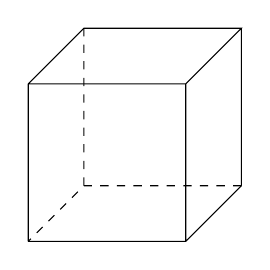
\begin{tikzpicture}[x=(-135:{0.5}),y=(0:1cm),z=(90:1cm),scale =2]
    \pgfmathsetmacro{\a}{1}
    \pgfmathsetmacro{\b}{1}
    \pgfmathsetmacro{\c}{1}

    \coordinate (A) at (\a,0,0);
    \coordinate (B) at (\a,\b,0);
    \coordinate (C) at (0,\b,0);
    \coordinate (D) at (0,0,0);
    \coordinate (A1) at (\a,0,\c);
    \coordinate (B1) at (\a,\b,\c);
    \coordinate (C1) at (0,\b,\c);
    \coordinate (D1) at (0,0,\c);

    % \foreach \x in {A,B,C,D,A1,B1,C1,D1}{
    %     \filldraw (\x)  circle (1pt) node {$\x $};
    % }
    \draw (A) -- (B)-- (C) (A1)--(B1)--(C1)--(D1)--(A1) (A)--(A1) (B)--(B1) (C)--(C1);
    \draw[dashed] (C) --(D) --(A)(D)--(D1);

\end{tikzpicture}



\end{document}